\chapter[Microcontroladores]{Microcontroladores}

\section{O que é um microcontrolador}

De maneira prática, um microcontrolador é um pequeno computador capaz de executar instruções pré-programadas, entretanto é construído em apenas um circuito integrado que contém todos os subsistemas necessários para seu funcionamento, dentre eles a unidade de processamento central (CPU, sigla para Central Processing Unit), a memória e os periféricos programáveis de entrada e saída % \cite{Basics2008}.

\begin{figure}[h!]
  \centering
  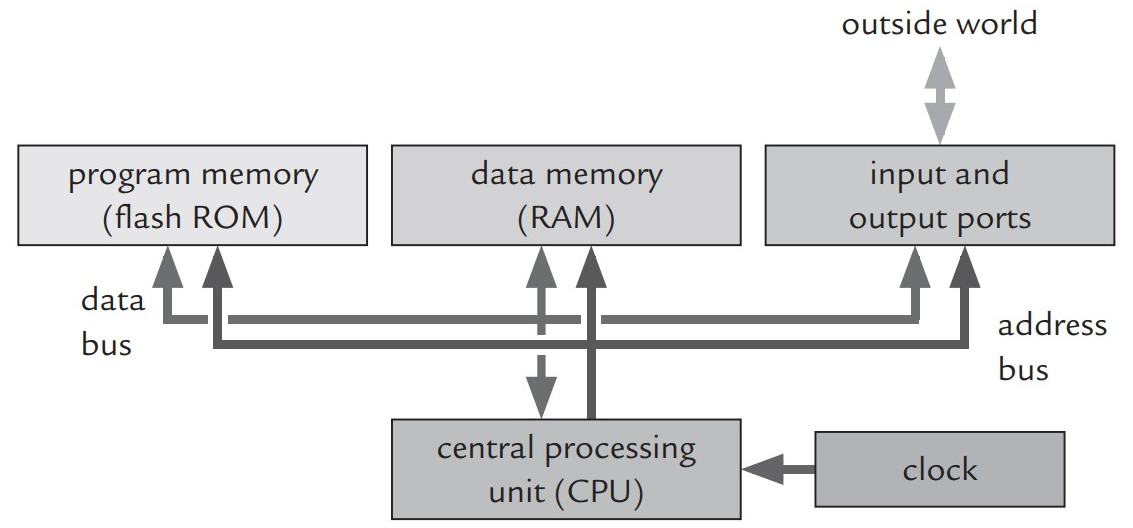
\includegraphics[width=0.9\linewidth]{figuras/componentes-microcontrolador.png}
  \caption{Subsistemas básicos de um microcontrolador.}
  \label{fig:arq_micro}
\end{figure}

\subsection{Unidade de processamento central}

Responsável por executar efetivamente as operações, este subsistema conta com os seguintes componentes:

\textbf{Unidade lógica aritmética (ULA)}: Realiza os cálculos necessários nas operações, embora cada microntrolador possa apresentar diferentes conjuntos de instruções, operações básicas como soma, subtração, AND, OR e deslocamento de bits são alguns dos exemplos de funções que as ALUs podem fazer.

\textbf{Registadores}: Além de fornecerem espaço para as informações básicas de operação da CPU como o program couter (PC), stack poiter (SP) e status register (SR). Além disso os registadores são responsáveis por armazenar resultados temporários.

\textbf{Outros}: Diversos outros componentes para decodificar instruções, manipular resets e interrupções.

\subsection{Memória}

Embora os registradores também sejam responsáveis por armazenar dados, a memória é um componente dedicado exclusivamente para essa função.

\textbf{ROM:} A memória somente de leitura ou ROM (acrônimo em inglês de \textit{read-only memory}), responsável por armazenar o programa gerado. As memórias ROM se encaixam na categoria não-voláteis, pois são capazes de reter as informação mesmo quando a energia é removida. Apesar do nome, atualmente os microcontroladores por escrever dados na memória ROM, entretanto esse processo é mais complicado e lento do que na memórias RAM.

\textbf{RAM:} A memória de acesso aleatório (do inglês \textit{Random Access Memory}) normalmente amazenam os dados gerados durante a execução do programa e são mais rápidas que a ROM. Geralmente do tipo voláteis, ou seja, perdem-se todos os dados na falta de energia, embora o nome sugira, o acesso aleatório não é exclusivo das memórias RAM.

\subsection{Input e Output}

Ponto fundamental dos microcontroladores, estes componentes são responsáveis por fornecer comunicação com o mundo exterior, podendo se dar de maneira digital e/ou analógica em alguns microcontroladores.

\subsection{Barramentos de endereço e dados}

A comunicação entre todos os componentes acontece a todo momento e a velocidades muitos altas, para tornar isso possível é necessário criar essa ligações.

\subsection{Clock}

Praticamente todos os sistemas digitais necessitam de um clock para funcionarem, e é neste componente onde isso é gerado, normalmente	é obtido por um cristal ou fonte externa. Atualmente os microcontroladores são capazes de trabalhar com uma faixa relativamente grande de frequências.

\subsection{Temporizadores}

Como uma extensão dos clocks, os temporizadores são muito versáteis e necessários para diversas funções do microcontrolador.

\textbf{Watchdog Timer:} Como ferramenta de segurança esse contador é responsável por resetar o microcontrolador caso o programa entre em um loop infinito.

\subsection{Interfaces de comunicação}

Ampliando a função de Input e Output, as interfaces de comunicação fornecem protocolos próprios para a transmissão de dados buscando sempre transmitir de maneira rápida e com baixas taxas de perda, dentre as mais comuns presentes nos microcontroladores temos como exemplo a Serial Peripheral Interface (SPI), Inter-Integrated Circuit (I2C) e Universal Asynchronous Receiver/Transmitter (UART).

\subsection{Conversores}

Dados do mundo exterior são essencialmente analógica e para tornar a interação com circuitos que trabalham dessa maneira os conversores são peça indispensável. Essa conversão pode acontecer em dois sentidos, convertendo um sinal analógico em digital (A/D) e vice-versa (D/A).

\section{Software}

A programação de um microcontrolador percorre diversos níveis de forma a converter o código escrito para a linguagem de máquina.

\subsection{Linguagem de Máquina}

A linguagem de máquina consiste em um código binário que o processador consegue entender. No início da computação a programação era feita dessa forma, mas hoje em dia não é mais necessário trabalhar nessa linguagem de baixo-nível.

\subsection{Assembly}

Um nível um pouco, só um pouco, acima da linguagem de máquina temos o assembly, esta linguagem traduz o código binário para algumas palavras conhecidas como mnemónicos.

Uma grande desvantagem do  é que essa tradução de código binário depende diretamente do processador, ou seja, cada tipo de processador tem um dicionário de palavras único. Em compensação ao utilizar o assembly consegue-se ter mais controle sobre a eficiência do código e, além disso, é possível ver exatamente o comportamento de processador no processo de debug.

\subsection{Linguagem C}

Uma das linguagem de programação mais usadas para a programação de microcontroladores, por ser uma linguagem de alto-nível é possível criar lógicas complexas sem muito trabalho e sem a necessidade de conhecer todo conjunto de instruções do processador.
A desvantagem fica por conta da compilação que pode não ser a mais eficiência, embora atualmente os compiladores estão cada vez melhores e trabalham muito bem esse ponto.

\section{Aplicações}

Microcontroladores são utilizados em praticamente qualquer dispositivo automatizado, isso pode incluir sistemas de controle de automóvel, dispositivos médicos implantáveis, controles remotos, máquinas de escritório, eletrodomésticos, ferramentas elétricas, brinquedos, entre muitos outros.

São diversos pontos que contribuem para sua grande ...

\section{Uso na educação}
\label{sec:educacao}
